\documentclass{article}
\usepackage{graphicx} % Required for inserting images
\usepackage{graphicx} % Required for inserting images
%\usepackage[left=0.5in, right=0.5in, top=0.5in, bottom=0.5in]{geometry}
\usepackage[left=1.5cm, right=1.5cm, top=0.5cm, bottom=1.5cm]{geometry}
\usepackage{amsmath}
\usepackage{amssymb}
\usepackage{amsfonts}
\usepackage{amsthm}
\usepackage{ulem}
\usepackage{bm}
\usepackage{tikz}

\date{}

\begin{document}
\fontsize{13}{15} \selectfont %This is 13pt text with 15pt line spacing.

\begin{center}
 \text{Potterhouse School: \hspace{1cm} Place Value 5.} \qquad \\ 
\end{center} \\ 

Name: ........................................................................ \hspace{0.5cm}  Date: ....................... \hspace{0.5cm}  Class: ......

\par
\vspace*{10pt} 
\textit{(You must show your working.)  }
\vspace{10pt}

\hline
\vspace{10pt}

\par
\text{(1) What is 7584043 rounded to the nearest ten thousand? } \\
\vspace*{20pt}
\par

\begin{flushright}
    \text{(2)}
\end{flushright}
 \vspace{10pt}

\hline
\vspace{10pt}

\par
\text{(2) Write these numbers in order of size. Start with the smallest. } \\

8.405 \hspace{3cm} 8.504  \hspace{3cm} 85.04 \hspace{3cm} 850.04 \hspace{3cm} 8.045 
\vspace{30pt}

 ..... \hspace{3cm} ..... \hspace{3cm}  ..... \hspace{3cm} ..... \hspace{3cm} .....  

\par
\text{smallest} 
\vspace{10pt}

\begin{flushright}
    \text{(2)}
\end{flushright}
 \vspace{10pt}

\hline
\vspace{10pt}

\par
\text{(3) Write these numbers in order of size. Start with the smallest. } \\

0.075 \hspace{3cm} 0.75 \hspace{3cm} 57\% \hspace{3cm}  \( \displaystyle \frac{5}{7} \) 
\vspace{70pt}

 ..... \hspace{3cm} ..... \hspace{3cm}  ..... \hspace{3cm} .....     \\

 smallest
 
 \begin{flushright}
    \text{(2)}
\end{flushright}
 
 \vspace{10pt}
 \hline
 \vspace{10pt}

\text{(4) What does 9 represent in this number?   } \\
 \[ 94283.82 \]
 
\begin{center}
\begin{tabular}{c@{\hspace{3cm}}c@{\hspace{3cm}}c@{\hspace{3cm}}c}
  Ones & Ten Thousands & Hundredths & Tenths \\
  \includegraphics[width=1cm]{cross.png} & 
  \includegraphics[width=1cm]{cross.png} & 
  \includegraphics[width=1cm]{cross.png} & 
  \includegraphics[width=1cm]{cross.png} \\
\end{tabular}
\end{center}

\begin{flushright}
    \text{(2)}
\end{flushright}
 \vspace{10pt}
 \newpage

\text{(5) What is 50215 rounded to the nearest thousand? }
\begin{center}
\begin{tabular}{c@{\hspace{3cm}}c@{\hspace{3cm}}c@{\hspace{3cm}}c}
  50,200 & 51,000 & 50,000 & 50,020 \\
  \includegraphics[width=1cm]{cross.png} & 
  \includegraphics[width=1cm]{cross.png} & 
  \includegraphics[width=1cm]{cross.png} & 
  \includegraphics[width=1cm]{cross.png} \\
\end{tabular}
\end{center}

\begin{flushright}
    \text{(2)}
\end{flushright}
 \vspace{10pt}

 \hline
 \vspace{10pt}

\par
\begin{flushleft}
 \text{(6) Write} \textit{\textbf{six million, two hundred and forty-four thousand, five hundred and tweleve}} \\ \text{in digits.} 
 \end{flushleft}
 
 \par
 \vspace{30pt}
 ..............................................
\begin{flushright}
    \text{(2)}
\end{flushright}
 \vspace{10pt}

 \hline
 \vspace{10pt}

 \text{(7) Write} \bm{\mathit{391004}} \text{in words. } 
 %\text{(7) Write} \text{\textit{$\bm{38127}$}} \text{in words. } 
 \par
 \vspace{30pt}

\noindent \dotuline{\hspace{18cm}} \\
\par
\noindent \dotuline{\hspace{18cm}} \\

\begin{flushright}
    \text{(2)}
\end{flushright}
 \vspace{10pt}

 \hline
 \vspace{10pt}

%\( \mathbf{\mathit{20}} \)

\text{(8) What is the value of the 8 in this number? }
\( 482706\)
\vspace{10pt}

\begin{center}
\begin{tabular}{c@{\hspace{3cm}}c@{\hspace{3cm}}c@{\hspace{3cm}}c}
  8 & 80 & 80,000 & 800 \\  
  \includegraphics[width=1cm]{cross.png} & 
  \includegraphics[width=1cm]{cross.png} & 
  \includegraphics[width=1cm]{cross.png} & 
  \includegraphics[width=1cm]{cross.png} \\
\end{tabular}
\end{center}

\begin{flushright}
    \text{(2)}
\end{flushright}
 \vspace{10pt}

 \hline
 \vspace{10pt}

\text{(9) Fill in X and Y in the number line below. } 
\vspace{30pt}

 %%\begin{tikzpicture}
    % Draw the main line
   % \draw[->] (0,0) -- (10,0);
    
    % Draw tick marks and labels
   % \foreach \x/\label in {0/3000, 2/3200, 4/3400, 6/3600, 8/3800, 10/4000} {
    %    \draw (\x,-0.1) -- (\x,0.1);
        % Omit labels at positions 4 and 8 to leave them blank
     %   \ifnum\x=2 \else \ifnum\x=4 \ifnum\x=6 \ifnum\x=8  
      %      \node[below] at (\x,-0.2) {\label};
       % \fi\fi
    }
    
    % Draw letters 'X' and 'Y' at positions 4 and 8
  %  \node[below] at (2,-0.2) {X};
 %   \node[below] at (6,-0.2) {Y};
    
%\end{tikzpicture}

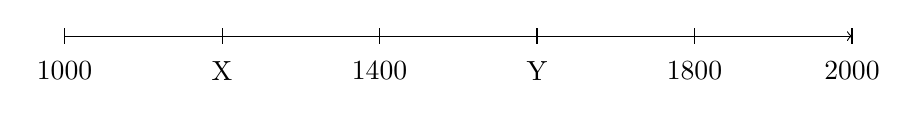
\begin{tikzpicture}
    % Draw the main line
    \draw[->] (0,0) -- (10,0);
    
    % Draw tick marks and labels
    \foreach \x/\label in {0/1000, 2/1200, 4/1400, 6/1600, 8/1800, 10/2000} {
        \draw (\x,-0.1) -- (\x,0.1);
        % Omit labels at positions 4 and 8 to leave them blank
        \ifnum\x=2 \else \ifnum\x=6 \else
            \node[below] at (\x,-0.2) {\label};
        \fi\fi
    }
    
    % Draw letters 'X' and 'Y' at positions 4 and 8
    \node[below] at (2,-0.2) {X};
    \node[below] at (6,-0.2) {Y};
    
\end{tikzpicture}

\begin{flushright}
    \text{(2)}
\end{flushright}
 \vspace{10pt}


\text{(10) Partition the number below.}  \\
$$ 745690 $$
\vspace{30pt}

\hline
\vspace{10pt}

%\item 
%\begin{align*}
%&\phantom{+}\underline{\phantom{00}1234} \\
%&\phantom{+}\underline{\phantom{0}0789} \\
%+&\underline{54321} \\
%&\text{------} \\
%&55644
%\end{align*}


\end{document}


